\documentclass{article}
\usepackage{graphicx}
\usepackage{alltt}
\usepackage{amsmath}
\usepackage{amsfonts}
\usepackage{bigstrut}
\usepackage{enumerate}
\usepackage{fancyhdr}
\usepackage[top=.75in, bottom=.95in, left=.75in, right=.75in]{geometry}
\usepackage{float}
\usepackage{lastpage}
\usepackage{tikz}
\usepackage[latin1]{inputenc}
\usepackage{color}
\usepackage{array}
\usepackage{longtable}
\usepackage{calc}
\usepackage{multirow}
\usepackage{hhline}
\usepackage{ifthen}
\usepackage{listings}
\usepackage{circuitikz}
\usepackage{pgfplots}
\usepackage{hyperref}
\usepackage{tabto}
\usepackage{fancyvrb}
\usepackage{url}
%\lstset{language=VHDL,basicstyle=\ttfamily}
\definecolor{mygreen}{rgb}{0,0.6,0}
\definecolor{mygray}{rgb}{0.5,0.5,0.5}
\definecolor{mymauve}{rgb}{0.58,0,0.82}
\lstset{ %
  backgroundcolor=\color{white},   % choose the background color; you must add \usepackage{color} or \usepackage{xcolor}; should come as last argument
  basicstyle=\normalsize,        % the size of the fonts that are used for the code
  breakatwhitespace=false,         % sets if automatic breaks should only happen at whitespace
  breaklines=true,                 % sets automatic line breaking
  captionpos=b,                    % sets the caption-position to bottom
  commentstyle=\color{mygreen},    % comment style
  deletekeywords={...},            % if you want to delete keywords from the given language
  escapeinside={\%*}{*)},          % if you want to add LaTeX within your code
  extendedchars=true,              % lets you use non-ASCII characters; for 8-bits encodings only, does not work with UTF-8
  frame=single,	                   % adds a frame around the code
  keepspaces=true,                 % keeps spaces in text, useful for keeping indentation of code (possibly needs columns=flexible)
  keywordstyle=\color{blue},       % keyword style
  language=VHDL,                   % the language of the code
  morekeywords={*,...},            % if you want to add more keywords to the set
  numbers=left,                    % where to put the line-numbers; possible values are (none, left, right)
  numbersep=5pt,                   % how far the line-numbers are from the code
  numberstyle=\tiny\color{mygray}, % the style that is used for the line-numbers
  rulecolor=\color{black},         % if not set, the frame-color may be changed on line-breaks within not-black text (e.g. comments (green here))
  showspaces=false,                % show spaces everywhere adding particular underscores; it overrides 'showstringspaces'
  showstringspaces=false,          % underline spaces within strings only
  showtabs=false,                  % show tabs within strings adding particular underscores
  stepnumber=2,                    % the step between two line-numbers. If it's 1, each line will be numbered
  stringstyle=\color{mymauve},     % string literal style
  tabsize=2,	                   % sets default tabsize to 2 spaces
  title=\lstname                   % show the filename of files included with \lstinputlisting; also try caption instead of title
}
\floatstyle{plain}
\restylefloat{figure}
\pagestyle{fancy}
\fancyhead{}
\fancyfoot{}
\setlength{\headheight}{59.0pt}
\def\inputGnumericTable{}
\fancyhead[CO]{\textbf{Air Force Institute of Technology\\Department of Electrical and Computer Engineering\\
Distributed Software Systems (CSCE 689)}\\Homework 3\\Due Date: 10-February-2020}
\lhead{\today}
\rhead{2d Lt Josh Larson\\Page \thepage{} of \pageref{LastPage} }
%\newlength\tindent
%\setlength{\tindent}{\parindent}
%\setlength{\parindent}{0pt}
%\renewcommand{\indent}{\hspace*{\tindent}}
\setlength{\parskip}{\baselineskip}


\newcommand{\graphfromadj}[3][arc/.try]{
    \foreach [count=\r] \row in {#3}{
        \foreach [count=\c] \cell in \row{
            \ifnum\cell=1%
                \draw[arc/.try=\cell, #1] (#2\r) edge (#2\c);
            \fi
        }
    }
}

\newcommand{\weigthgraphfromadj}[3][draw,->]{
    \foreach [count=\r] \row in {#3}{
        \foreach [count=\c] \cell in \row{
            \if0\cell%
            \else
                \draw[arc/.try=\cell, #1] (#2\r) edge node[arc label/.try=\cell]{\cell} (#2\c);
            \fi
        }
    }
}

\begin{document}
\subsection*{Code Location}
Github Link: \url{https://github.com/Josh-Larson/AFIT-CSCE689-HW3-S}

\subsection*{Question 1}
As can be seen in the figure, performance levels off at eight threads--which is the number of hyperthreaded cores on my machine.  However the optimal thread count is 3 because of memory caching and contention issues between the spawend threads and the main threads.  After the optimal is slowly increases until the level-off point at 8 threads.

\begin{tikzpicture}
	\begin{axis}[
		title={Multi-Threaded Timing},
		xlabel={Thread Count},
		ylabel={Timing (s)},
		xmin=1, xmax=32,
		ymin=30, ymax=60,
		xtick={0,1,2,4,8,16,32},
		ytick={30,35,40,45,50,55,60},
		legend pos=north west,
		ymajorgrids=true,
		grid style=dashed,
	]
	 
	\addplot[
		color=blue,
		mark=square,
		]
		coordinates {
			(1,49.183940)
			(2,40.610726)
			(3,37.367224)
			(4,38.280318)
			(5,38.135054)
			(6,39.575609)
			(7,40.074504)
			(8,40.904750)
			(12,41.520712)
			(16,41.633111)
			(20,41.801025)
			(24,41.377079)
			(28,41.602486)
			(32,41.139662)			
		};
		\legend{4-core/8-thread machine}
	 
	\end{axis}
\end{tikzpicture}

\subsection*{Question 2}
Below is the max unsigned int evaluation for 5 trials.  There is a small variation between 40.1s and 41.5s, which can be accounted for by processor interruptions and possible cache misses spread out over a longer period of time.

\begin{tikzpicture}
	\begin{axis}[
		title={Max Unsigned Int Test With 5 Trials},
		xlabel={Trial},
		ylabel={Timing (s)},
		xmin=0, xmax=6,
		ymin=40, ymax=42,
		xtick={1,2,3,4,5},
		ytick={40,40.5,41,41.5,42},
		legend pos=north west,
		ymajorgrids=true,
		grid style=dashed,
	]
	
	\addplot[
		color=blue,
		mark=square,
	]
	coordinates {
		(1,40.181108)
		(2,40.982484)
		(3,40.859609)
		(4,41.474213)
		(5,40.386814)
	};
	\legend{8-thread machine w/ 8 running threads}
	\end{axis}
\end{tikzpicture}

\end{document}
